\documentclass[11pt]{article}
\usepackage{amsmath,amssymb,amsfonts,latexsym,graphicx,amsthm}
\usepackage{fullpage,color}
\usepackage{tikz}
\usetikzlibrary{calc}
\usetikzlibrary{intersections}
\usepackage[framemethod=tikz]{mdframed}
\usepackage{tikz-cd}

\begin{document}

		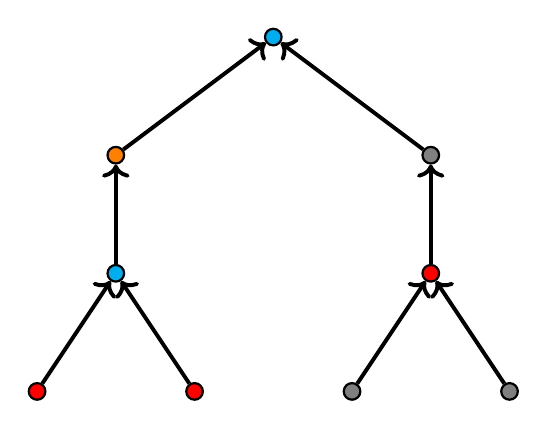
\begin{tikzpicture}[thick,scale=1]


	\draw (-3, 0) node(1)[circle, draw, fill=red, inner sep=0pt, minimum width=6pt] {};
	\draw (-1, 0) node(2)[circle, draw, fill=red, inner sep=0pt, minimum width=6pt] {};
	\draw (1, 0) node(3)[circle, draw, fill=black!50, inner sep=0pt, minimum width=6pt] {};
	\draw (3, 0) node(4)[circle, draw, fill=black!50, inner sep=0pt, minimum width=6pt] {};

	\draw (-2, 1.5) node(5)[circle, draw, fill=cyan, inner sep=0pt, minimum width=6pt] {};
	\draw (2, 1.5) node(6)[circle, draw, fill=red, inner sep=0pt, minimum width=6pt] {};

	\draw (-2, 3) node(7)[circle, draw, fill=orange, inner sep=0pt, minimum width=6pt] {};
	\draw (2, 3) node(8)[circle, draw, fill=black!50, inner sep=0pt, minimum width=6pt] {};

	\draw (0, 4.5) node(9)[circle, draw, fill=cyan, inner sep=0pt, minimum width=6pt] {};


	\draw [->, line width = 0.5mm] (1) to (5);
	\draw [->, line width = 0.5mm] (2) to (5);
	\draw [->, line width = 0.5mm] (3) to (6);
	\draw [->, line width = 0.5mm] (4) to (6);
	\draw [->, line width = 0.5mm] (5) to (7);
	\draw [->, line width = 0.5mm] (6) to (8);
	\draw [->, line width = 0.5mm] (7) to (9);
	\draw [->, line width = 0.5mm] (8) to (9);

\end{tikzpicture}

\end{document}